\section{AdaBoost}

\begin{frame}{AdaBoost - How it works}
    \begin{itemize} \pause
        \item AdaBoost invokes the weak learner $T$ times
            on the training data using different sample weights
            $(D_1^{(t)}, ..., D_m^{(t)}), \  t=1, ..., T$ \pause
        \item In every iteration $t$, the weak learner finds a hypothesis $h_t$ \pause
        \item Then, AdaBoost does a weighted majority vote:
    \end{itemize}
    \begin{equation*}
        h(x) = \text{sign}\left( \sum_{t=1}^T w_t h_t(x) \right)
    \end{equation*} \pause
    Let's look at this in more detail...
\end{frame}

\begin{frame}{One iteration of AdaBoost}
    \begin{enumerate} \pause
        \item Invoke the weak learner on the training data weighted by $D^{(t)}$
        \begin{itemize}
            \item In iteration $t=1$, we use equal weights $D_i^{(t)}=\frac{1}{m}$
        \end{itemize} \pause
        \item Compute a weight for the resulting hypothesis $h_t$ like this:
        \begin{equation*}
            w_t = \frac{1}{2} \text{log} \left( \frac{1}{\epsilon_t} - 1 \right)
        \end{equation*}
        \begin{itemize}
            \item $\epsilon_t$ is the (weighted) training error of $h_t$ \pause
        \end{itemize}
        \item Update the weights $D_i^{(t)}$ like this
        \begin{equation*}
            D_i^{(t+1)} = \frac{D_i^{(t)} \text{exp} \left( -w_t y_i h_t(\mathbf{x}_i) \right)}{
        \sum_{j=1}^m D_j^{(t)} \text{exp} \left( -w_t y_j h_t(\mathbf{x}_j) \right) }
        \end{equation*}
    \end{enumerate}
\end{frame}

\begin{frame}{A step by step example\footnote{Taken from the book \textit{Boosting: Foundations and Algorithms} written by Freund and Schapire~\cite{boosting}.
You can read it for free at \url{https://mitpress.mit.edu/books/boosting}}}
    \begin{figure}
        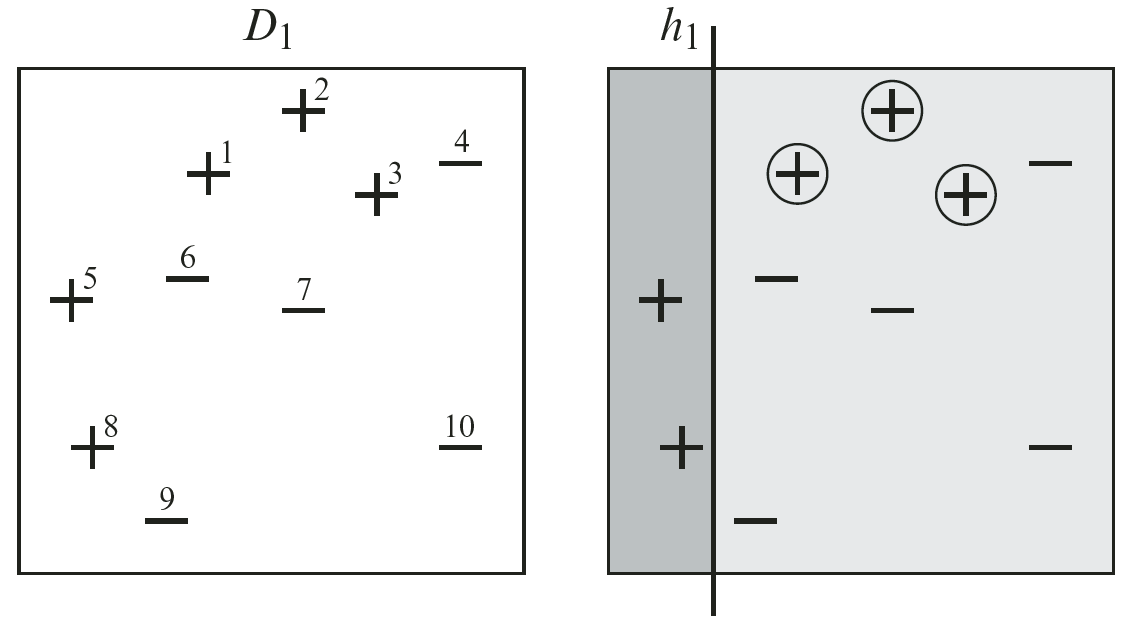
\includegraphics[width=\textwidth]{img/example_1}
    \end{figure}
\end{frame}

\begin{frame}{A step by step example}
    \begin{figure}
        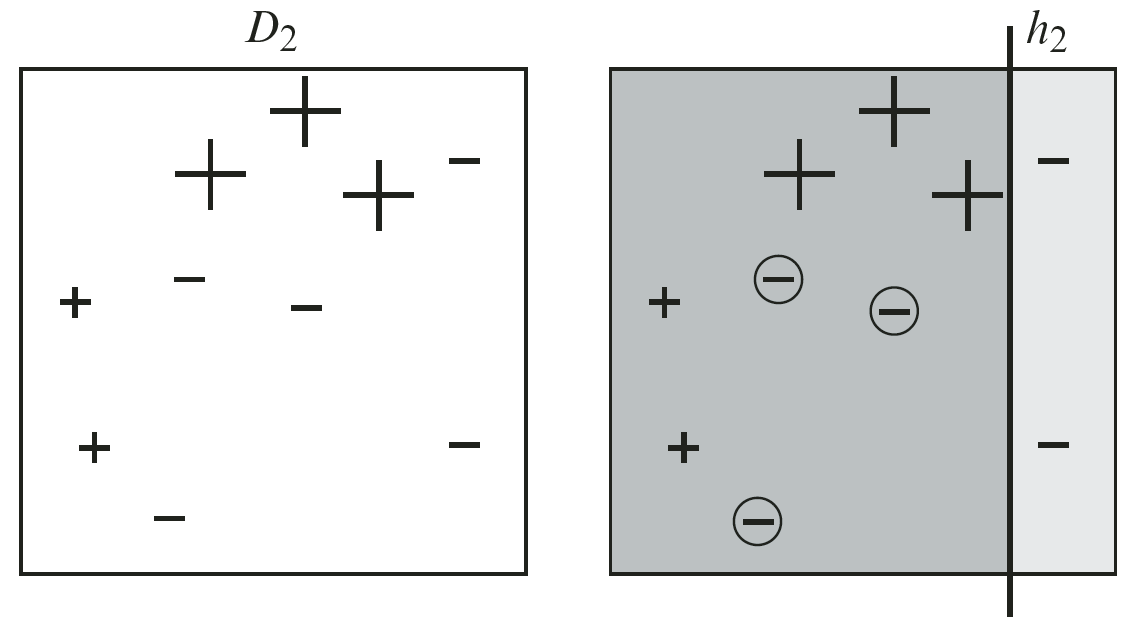
\includegraphics[width=\textwidth]{img/example_2}
    \end{figure}
\end{frame}

\begin{frame}{A step by step example}
    \begin{figure}
        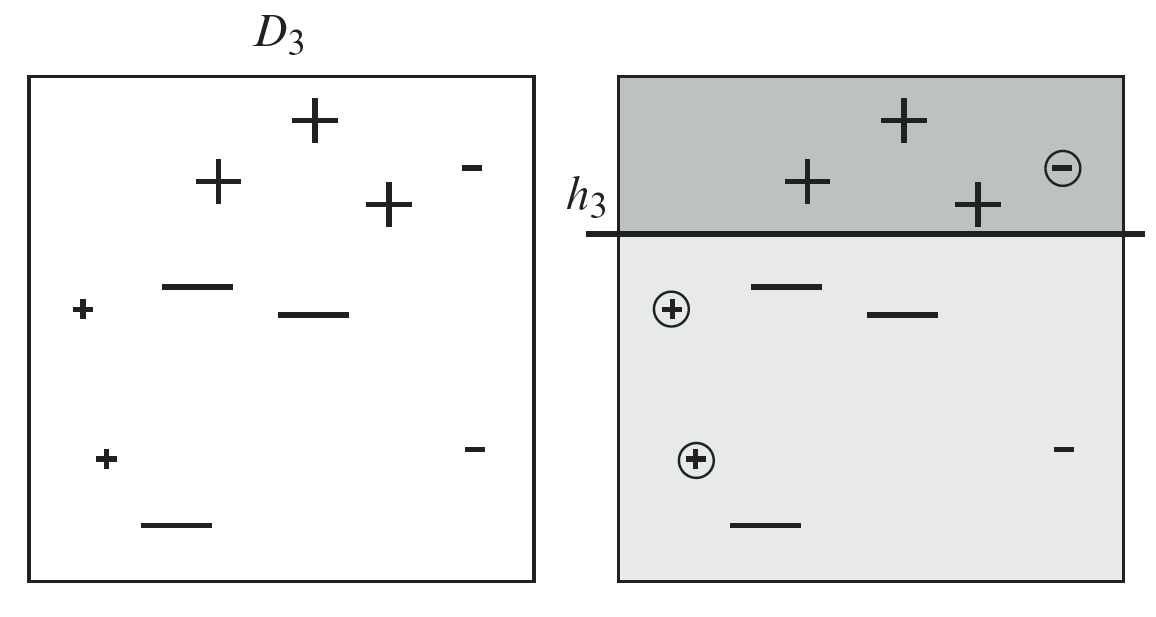
\includegraphics[width=\textwidth]{img/example_3}
    \end{figure}
\end{frame}

\begin{frame}{A step by step example}
    \begin{figure}
        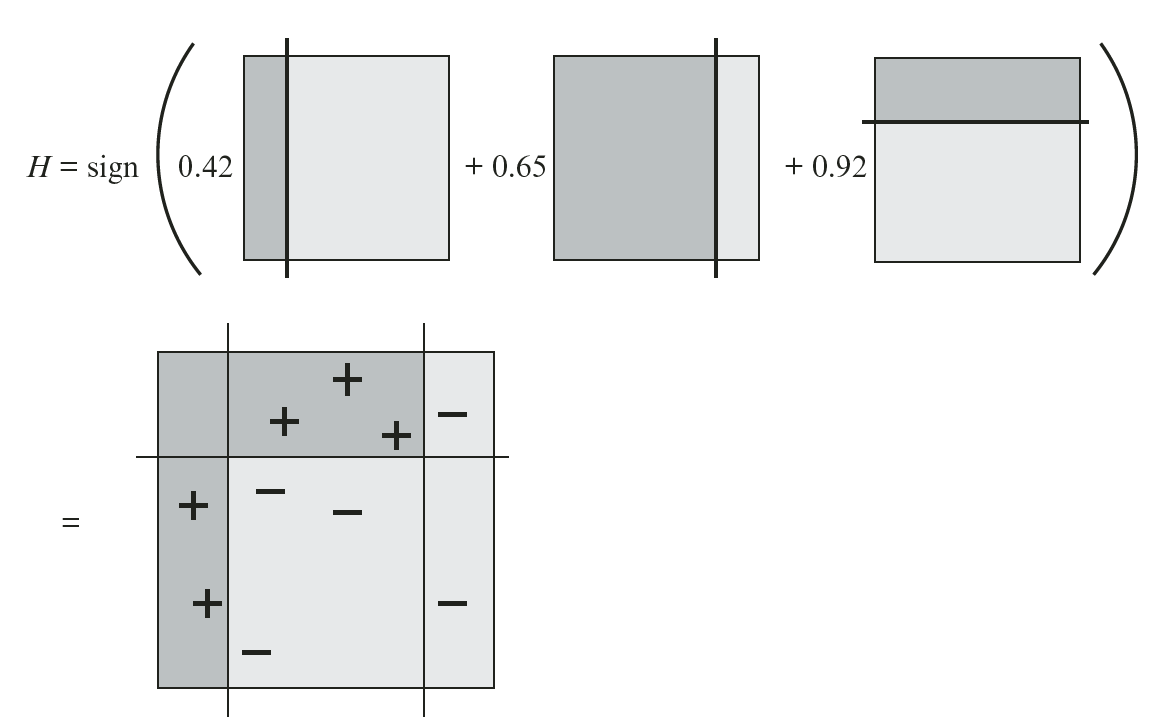
\includegraphics[width=\textwidth]{img/example_result}
    \end{figure}
\end{frame}

\begin{frame}{AdaBoost training error}
    \begin{itemize} \pause
        \item In the previous example, the training error was efficiently reduced to zero
        \begin{itemize}
            \item If the weak learner is efficient, then AdaBoost is efficient
        \end{itemize} \pause
        \item What about the general case? \pause
        \begin{equation*}
            L_S(h) = \frac{1}{m} \sum_{i=1}^m \mathds{1}_{\left[ h(\mathbf{x}_i) \neq y_i \right]} \leq e^{-2 \gamma^2 T}
        \end{equation*} \pause
        \item The training error of AdaBoost decreases exponentially in $T$ \pause
    \end{itemize}
    \textbf{...but what about the out of sample error?}
\end{frame}

\begin{frame}{AdaBoost hypothesis class}
    \begin{itemize} \pause
        \item The AdaBoost hypothesis is part of the following class:
        \begin{equation*}
            L(B, T) = \left \{ x \mapsto \text{sign} \left( \sum_{t=1}^T w_t h_t(x) \right): \ 
        w \in \mathbb{R}^T, \  h_t \in B \right \}
        \end{equation*} \pause
        \item It can be shown that VC dim of $L(B, T)$ is in 
            $\mathcal{O}(T \cdot \text{VCdim}(B))$ \pause
        \item For decision stumps, VC dim is finite \pause
        \begin{itemize}
            \item[$\Rightarrow$] VC dim of AdaBoost hypothesis is finite! $L(B, T)$ is learnable!
        \end{itemize} \pause
        \item $T$ controls model complexity ($\rightarrow$ B/C tradeoff)
        \begin{itemize}
            \item But what about overfitting?
        \end{itemize}
    \end{itemize}
\end{frame}